\section{Additional Experimental Details}
\label{app:experimental-details}

% NOTE: This appendix is intended to be pasted after the main experimental
% section. It records implementation-level details that are useful for
% reproducibility but would otherwise distract from the main claims in Section 4.

\paragraph{Synthetic generator.}
Each synthetic instance is generated from a latent linear--Gaussian model. We
sample a latent vector $s \in \mathbb{R}^{r_\star}$ and observe
\[
    z = C s + \sigma_z \epsilon_z,
    \qquad
    y_k = a_k^\top s + \sigma_y \epsilon_k,
\]
where $C \in \mathbb{R}^{D_x \times r_\star}$ is a randomly sampled
orthonormal context operator, $a_k$ is the $k$th target direction, and the noise
terms are independent isotropic Gaussians. Thus the population predictive
structure is known, but the context coordinates are not aligned with the
canonical basis.

% NOTE: The random orthonormal C avoids the degenerate identity-coordinate case
% while preserving a clean ground-truth predictive subspace for measuring
% recovery.

\paragraph{Target banks.}
The target operators are constructed in latent space. In the saturation and
bottleneck experiments, we use a complementary target bank whose directions
progressively cover the $r_\star$ latent predictive coordinates. In the
heterogeneity experiment, the construction parameter is chosen so that the
induced population heterogeneity level $\lambda_{\mathrm{het}}$ is sampled
approximately evenly; the plot therefore uses the measured heterogeneity level
directly on the horizontal axis. In the overlap experiment, the overlap
parameter concentrates target mass onto shared latent directions, reducing the
effective diversity of the target bank.
In the predictive-isotropy ablation, the target bank is constructed to control
the spectrum directly. For a spectrum decay parameter $\rho\in(0,1]$, we set
\[
    A^\top A
    =
    Q\operatorname{diag}(\lambda_1,\ldots,\lambda_d)Q^\top,
    \qquad
    \lambda_i
    =
    \tau\frac{\rho^{i-1}}{\sum_{j=1}^d\rho^{j-1}},
\]
where $Q$ is a random orthogonal rotation and $\tau$ is fixed across all
conditions. Thus $\operatorname{rank}(A)=d$ and
$\operatorname{tr}(A^\top A)=\tau$ are unchanged, while the predictive spectrum
ranges from flat ($\rho=1$) to strongly anisotropic. Since the context operator
has orthonormal columns and $\sigma_z$ is fixed, this fixes the nonzero spectrum
of $H_K=T_K^\top T_K$ up to the same scalar context-noise factor across all
conditions.

% INTERPRETATION: Heterogeneity and overlap are separated experimentally.
% Heterogeneity uses lambda_het as the primary x-axis; overlap keeps the
% redundancy parameter as the intervention and reports its effect on lambda_het.

\paragraph{Models and estimators.}
We first estimate the unrestricted linear predictor by ordinary least squares
and then compute its rank-$d$ reduced-rank regression approximation by
truncating the singular spectrum. The learned BM-JEPA linear predictor is
therefore the best rank-constrained linear map induced by the finite training
sample. Population curves use the corresponding population cross-covariance
operator under the same target bank and bottleneck dimension.

\paragraph{Metrics.}
All paper-facing MSE panels report average per-target test mean-squared error,
matching the normalization of $\mathcal R_K$ in \eqref{eq:per_target_risk}.
The CSV files also retain fixed-bank diagnostics on a common rich evaluation
target bank as auxiliary representation probes, but these are not the main
risk quantities used in the theory-facing panels. In \cref{fig:heterogeneity},
we show both quantities because they answer different questions: per-target
$\mathcal R_K$ evaluates the changing target bank used for training, whereas
fixed-bank MSE evaluates the recovered subspace on a common rich target bank.
As heterogeneity increases, $\mathcal R_K$ can remain nearly constant or rise
slightly because the task becomes less redundant; the fixed-bank probe can
decrease at the same time because the recovered subspace becomes more complete.
The standard-error band of $\mathcal R_K$ also shrinks as target coverage spreads
across more latent directions, so the per-target average becomes less dominated
by a single shared direction.
In \cref{fig:predictive-isotropy}, panel (e) uses a related common-bank probe:
after estimating the top-$d$ right singular subspace of the whitened operator
$\widehat T_K$, we fit a linear predictor from that recovered subspace to a
fixed flat evaluation target bank. This common-bank excess MSE is not a new
training objective; it is a representation diagnostic showing whether the
recovered predictive subspace captures all latent directions equally well.
Panel (f) keeps the canonical training-bank per-target MSE to show that total
predictive energy is controlled.
For the embedding-versus-predictive isotropy diagnostic, we additionally assign
a synthetic embedding covariance spectrum with eigenvalues proportional to
$\rho_{\mathrm{emb}}^{i-1}$ and fixed trace. This embedding spectrum is varied
independently of the predictive spectrum of $H_K$. It should therefore be read
as a controlled proxy for embedding-level isotropy diagnostics, not as a second
training objective.
Recovered rank is the effective numerical rank of the learned predictor,
computed using a relative singular-value threshold of $0.05$ times the leading
singular value. The heterogeneity metric $\lambda_{\mathrm{het}}$ is the
$r_\star$th nonzero eigenvalue of the target-induced Gram operator. In the
latent coordinates this is the same nonzero spectrum as $A^\top A$; in the
observed context coordinates it is the same nonzero spectrum as
$\Sigma_{ZY}\Sigma_{YZ}$ because $C^\top C=I$. Subspace error is measured by
the largest principal-angle sine between the recovered and true predictive
subspaces.
For the heterogeneity recovery bound, we also compute the empirical
perturbation $\widehat{\epsilon}=\|\widehat{\Sigma}_{YZ}-\Sigma_{YZ}\|_{\rm op}$
and the corresponding Davis--Kahan/Wedin-style denominator
$\sqrt{\lambda_{\mathrm{het}}}-\widehat{\epsilon}$. When this denominator is
nonpositive, the finite-sample bound is vacuous. We keep these quantities in
the CSV as validity diagnostics, but omit them from
\cref{fig:heterogeneity} because the bound is loose for this sweep and is
less informative than the rank and risk panels. The sharper recovery-bound
visualization appears in the post-saturation experiment, where the relative
conditioning condition is non-vacuous over the main finite window.

For the bottleneck experiment, the plotted spectral-tail quantity is the
reduced-rank approximation error predicted by the bottleneck spectral-tail
result:
\[
    \mathcal{E}_{\mathrm{tail}}(d)
    =
    \sum_{j>d} \sigma_j^2,
\]
where $\{\sigma_j\}$ are singular values of the relevant whitened regression
operator. In the figure we report the normalized ratio
$\mathcal{E}_{\mathrm{tail}}(d)/\sum_j\sigma_j^2$ and compare it with the
correspondingly normalized observed excess risk of the rank-$d$ estimator over
the unrestricted OLS estimator.

The rank panel in the bottleneck figure reports the effective rank of the
learned reduced-rank predictor, not the rank of the stacked cross-covariance.
The latter is fixed by the target bank and therefore does not change when the
bottleneck dimension is swept. Since the synthetic target bank has latent
predictive rank $r_\star=16$, a well-estimated rank-$d$ predictor is expected to
use approximately $\min\{d,r_\star\}$ directions. This panel is therefore a
sanity check that the bottleneck cap is the active rank constraint before
$d=r_\star$ and that additional capacity is unused afterward.

% NOTE: The spectral-tail curve is not an additional fitted model. It is
% computed directly from the singular spectrum and compared with observed
% excess risk.

\paragraph{Baselines.}
The main finite-sample baseline is unrestricted OLS, which removes the
embedding bottleneck. Population curves are included as reference predictions
for the same synthetic distribution. The bottleneck experiment additionally
reports a plug-in spectral tail computed from the finite-sample OLS spectrum,
allowing the risk decomposition to be checked using learned empirical
quantities rather than only population quantities.

\paragraph{Configuration summary.}
We list the main Phase-1 configurations used for the reported figures in
\cref{tab:appendix-configs}.

\begin{table}[t]
\centering
\caption{Phase-1 synthetic experiment configurations.}
\label{tab:appendix-configs}
\begin{tabular}{lcccccc}
\hline
Experiment & $n_{\mathrm{train}}$ & $n_{\mathrm{test}}$ & $r_\star$ & $K$ & $d$ & Noise \\
\hline
$K$ saturation & $256$ & $8192$ & $16$ & sweep & $16$ & $0.12$ \\
Heterogeneity & $32768$ & $8192$ & $16$ & $32$ & $16$ & $0.10$ \\
Overlap & $1024$ & $8192$ & $16$ & $24$ & $16$ & $0.08$ \\
Bottleneck & $96$ & $8192$ & $16$ & $32$ & sweep & $0.16$ \\
Post-saturation & $5000$ & $8192$ & $12$ & sweep & $12$ & $0.25$ \\
Predictive isotropy & $512$ & $8192$ & $16$ & $16$ & $16$ & $0.25$ \\
Embedding vs. predictive isotropy & $512$ & $8192$ & $16$ & $16$ & $16$ & $0.25$ \\
\hline
\end{tabular}
\end{table}

\paragraph{Additional theory diagnostics.}
The CSV schema also records the effective rank of the learned RRR coefficient,
the finite-sample target value $\min\{d,\widehat{r}_\star(K)\}$ predicted by
the rank identity, and their difference. This directly checks the rank identity beyond
the displayed rank of the stacked cross-covariance.

The diagnostic in \cref{fig:post-saturation} tests the post-saturation
relative-conditioning mechanism. The target bank is full rank from
$K^\star=d=12$ onward, so
additional targets do not change $r_\star(K)$. The relevant post-saturation
conditioning ratio is
\[
    \kappa_K^2
    =
    \frac{\lambda_d(H_K)}{\lambda_1(H_K)},
    \qquad
    H_K=T_K^\top T_K,\quad
    T_K=\Sigma_{YZ}^{(K)}\Sigma_{ZZ}^{-1/2}.
\]
The initial saturated target bank is deliberately imbalanced. Writing
$A_K^\top A_K$ for the latent target-bank design Gram, we initialize
\[
    A_{K^\star}^\top A_{K^\star}
    =
    Q\operatorname{diag}(c_1,\ldots,c_{12})Q^\top,
\]
where $Q$ is a fixed random orthogonal rotation and
\[
    (c_1,\ldots,c_{12})
    \approx
    (1.00,0.70,0.49,0.34,0.24,0.17,0.12,0.083,0.058,0.041,0.029,0.020).
\]
Thus the bank is already rank-$12$, but
$\kappa_{K^\star}^2\approx 0.02$. For $K>K^\star$, each additional target row
is added to the currently weakest eigendirection and contributes $0.1$ units of
target energy. This keeps $r_\star(K)=d$ throughout the plotted window while
increasing $\kappa_K^2$. The finite-sample subspace error and per-target excess
MSE decrease over the same window, supporting the repaired post-saturation
claim that extra targets help only when they improve relative conditioning of
the already-accessible predictive subspace.
In \cref{fig:post-saturation}, we keep the core post-saturation diagnostics in
the first row: the weakest and top eigenvalues of $H_K=T_K^\top T_K$ in a
shared panel, the relative conditioning ratio $\kappa_K^2$, and the effective
dimension of $T_K$. The
second row reports the risk-stability bound, excess risk, and finite-sample
risk. The
effective-dimension panel checks that
$\operatorname{effdim}(T_K)$ remains bounded over the finite
window in the finite-window post-saturation relative-geometry condition. To instantiate the
risk-stability constant, we compute the empirical ratio
\[
    \widehat L_K
    =
    \frac{[\widehat{\mathcal R}_K-\mathcal R_K^\star]_+}
    {\|\sin\Theta(V_K,\widehat V_K)\|_{\mathrm{op}}},
\]
using per-target excess MSE in the numerator, and set
$\widehat L=\max_{K,\mathrm{seed}}\widehat L_K$. Panel (d) then plots the
excess-risk left-hand side against the empirical bound curve
$\widehat L\|\sin\Theta(V_K,\widehat V_K)\|_{\mathrm{op}}$, matching the form of
the normalized risk-stability condition. Each seed is one
deterministic draw of the synthetic data and target bank, and the same
$\widehat L$ is used across the full plotted window. In the current run this
gives $\widehat L=6.94\times10^{-3}$.

For the concentration constant in \eqref{eq:post_saturation_epsilon}, we set
$\delta=0.1$ and compute
\[
    a_K
    =
    \sqrt{\frac{\operatorname{effdim}(T_K)+\log(1/\delta)}{n}},
    \qquad
    \widehat{\eta}_K
    =
    \frac{\|\widehat T_K-T_K\|_{\mathrm{op}}}{\|T_K\|_{\mathrm{op}}}.
\]
We then set $\widehat C_{0.9}$ to the $90$th percentile, over all plotted
$(K,\mathrm{seed})$ pairs, of $\widehat{\eta}_K/a_K$. This gives
$\widehat C_{0.9}=1.49$ and covers $90/100$ normalized perturbation samples by
construction. Panel (e) uses the calibrated bound
\[
    \frac{2\widehat L\widehat C_{0.9}a_K}{\kappa_K}
\]
from \cref{cor:post_saturation_excess_risk_bound}. Panel (f) adds this term to
the population OLS risk estimate, matching the risk-decomposition bound in
\cref{cor:risk_decomposition}. In this post-saturation setting
$d=r_\star(K)$, so the spectral-tail term is zero up to numerical precision.

% TODO: Verify theory labels before final paste:
% cor:post_saturation_relative_rate should point to Corollary 3.3.1.
% cor:post_saturation_excess_risk_bound should point to Corollary 3.3.2.
% cor:risk_decomposition should point to Corollary 3.3.3.
% eq:post_saturation_half_gap should point to the half-gap condition for the
% simplified finite-window rate.
To check that the simplified rate is not vacuous in the plotted regime, we
evaluate the empirical analogue of the half-gap condition in
\eqref{eq:post_saturation_half_gap}. Define the normalized perturbation
\[
    \widehat{\eta}_K
    :=
    \frac{\|\widehat T_K-T_K\|_{\mathrm{op}}}
    {\|T_K\|_{\mathrm{op}}}.
\]
The condition $\widehat{\eta}_K\le \kappa_K/2$ holds on the seed-averaged curve
for every plotted $K$, and it holds seed-wise for all $100/100$ deterministic
runs. At the weakest endpoint $K=12$, where the target bank is deliberately
closest to the small-conditioning boundary, the whitened diagnostic still
remains below the half-gap threshold in all seeds.
Representative values are:
\[
\begin{array}{c|cccc}
K & \widehat{\eta}_{K,\mathrm{mean}} & \widehat{\eta}_{K,\max}
  & \kappa_K/2 & \mathrm{valid\ seeds} \\
\hline
12 & 0.0469 & 0.0543 & 0.0707 & 10/10 \\
16 & 0.0489 & 0.0545 & 0.1440 & 10/10 \\
96 & 0.0713 & 0.0808 & 0.4771 & 10/10
\end{array}
\]

As an appendix-only diagnostic, we also substitute the same
$\widehat C_{0.9}$ into the intermediate Wedin-style recovery bound from the
proof of \cref{cor:post_saturation_relative_rate}. This yields the dashed
subspace-recovery curve in
\cref{fig:post-saturation-recovery-bound}. The induced curve is conservative:
it covers all observed $\|\sin\Theta_T\|_{\mathrm{op}}$ values in the plotted
window, because the deterministic perturbation step is looser than the empirical
perturbation quantile.

\begin{figure}[t]
    \centering
    
\includegraphics[width=\linewidth]{figures/exp_post_saturation_recovery_bound.pdf}
    \caption{Empirical calibration of the concentration constant in
    $\epsilon_n$ from the post-saturation recovery proof.
    Panel (a) plots the normalized perturbation
    $\widehat{\eta}_K=\|\widehat T_K-T_K\|_{\mathrm{op}}/\|T_K\|_{\mathrm{op}}$
    against the calibrated concentration bound
    $\widehat C_{0.9}\sqrt{(\operatorname{effdim}(T_K)+\log(1/\delta))/n}$.
    Panel (b) substitutes the same $\widehat C_{0.9}$ into the Wedin-style
    subspace-recovery bound and compares it with
    $\|\sin\Theta_T(V_K,\widehat V_K)\|_{\mathrm{op}}$.}
    \label{fig:post-saturation-recovery-bound}
\end{figure}

\paragraph{Predictive-isotropy construction.}
The fixed-trace predictive-isotropy experiment is designed to test the
operator-level Gaussianity claim without changing rank or total signal energy.
All conditions use $D_x=32$, $r_\star=d=K=16$,
$\sigma_z=\sigma_y=0.25$, and
$\operatorname{tr}(H_K)=15.06$ after the common whitening/context-noise scaling.
The decay values are
\[
    \rho\in\{1.00,\,0.85,\,0.65,\,0.45\}.
\]
They induce the following population diagnostics:
\[
\begin{array}{c|cccc}
\rho & \kappa_K^2(T_K) & \mathrm{entropy\ gap}
& \|\sin\Theta_T\|_{\mathrm{op}} & \mathrm{common\ excess\ MSE} \\
\hline
1.00 & 1.0000 & 0.000 & 0.136 & 2.96{\times}10^{-4} \\
0.85 & 8.74{\times}10^{-2} & -0.266 & 0.159 & 3.74{\times}10^{-4} \\
0.65 & 1.56{\times}10^{-3} & -1.507 & 0.497 & 2.79{\times}10^{-3} \\
0.45 & 6.27{\times}10^{-6} & -3.814 & 0.988 & 9.14{\times}10^{-2}
\end{array}
\]
The trace column is omitted because it is constant by construction. The strong
anisotropy settings intentionally violate the half-gap condition; they are
included to show the transition from the finite-window perturbative regime to
the nearly unrecoverable weak-direction regime. The flat and mild settings
satisfy the half-gap diagnostic in all seeds for the current sample size.

\cref{fig:predictive-isotropy-scatter} reports the same experiment as a
seed-level scatter. The points lie on the expected monotone trend: more
negative entropy gap, or smaller $\kappa_K^2(T_K)$, corresponds to larger
common-bank excess MSE.

\begin{figure}[t]
    \centering
    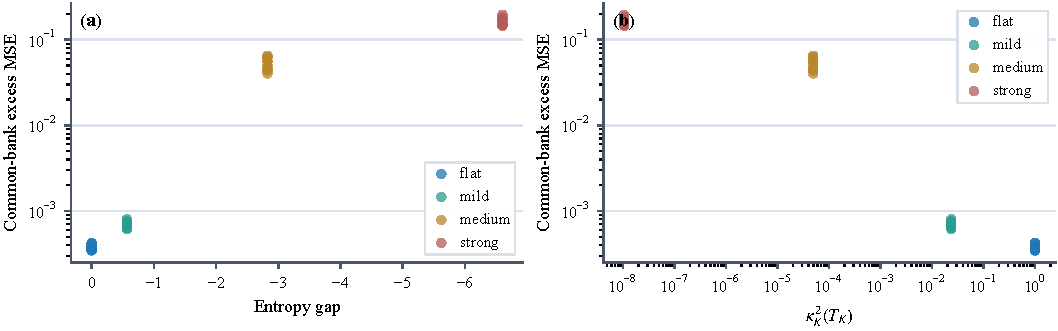
\includegraphics[width=\linewidth]{figures/exp_predictive_isotropy_scatter.pdf}
    \caption{Seed-level predictive-isotropy scatter. Each point is one
    deterministic seed and one fixed-trace spectrum condition. The common-bank
    excess MSE rises as the predictive spectrum becomes less isotropic, whether
    isotropy is measured by the log-determinant entropy gap or by
    $\kappa_K^2(T_K)$.}
    \label{fig:predictive-isotropy-scatter}
\end{figure}

\paragraph{Embedding versus predictive isotropy.}
The embedding-versus-predictive diagnostic varies two spectra independently:
the synthetic embedding covariance spectrum and the predictive spectrum of
$H_K=T_K^\top T_K$. The embedding decay values are
$\rho_{\mathrm{emb}}\in\{1.00,0.65,0.45\}$, and the predictive decay values are
$\rho_{\mathrm{pred}}\in\{1.00,0.85,0.65,0.45\}$. Both spectra are normalized to
the same trace within their own space. This creates cases with nearly isotropic
embedding covariance but badly conditioned predictive operator, and cases with
anisotropic embedding covariance but well-conditioned predictive operator.

\cref{fig:embedding-vs-predictive-isotropy} reports the result. Averaging over
predictive spectra, the common-bank excess MSE is unchanged across the three
embedding decay values. Averaging over embedding spectra, the same excess MSE
varies by orders of magnitude across predictive decay values:
\[
\begin{array}{c|c}
\rho_{\mathrm{pred}} & \mathrm{common\ excess\ MSE} \\
\hline
1.00 & 2.96{\times}10^{-4} \\
0.85 & 3.74{\times}10^{-4} \\
0.65 & 2.79{\times}10^{-3} \\
0.45 & 9.14{\times}10^{-2}
\end{array}
\]
The Spearman correlation between embedding entropy gap and common-bank excess
MSE is $0.00$ in this controlled grid, while the corresponding correlation for
predictive entropy gap is $-0.91$. This does not claim that embedding isotropy
is useless in nonlinear JEPA training; it shows that embedding isotropy is not
the operator-level quantity appearing in the finite-sample recovery bound.

\begin{figure}[t]
    \centering
    
\includegraphics[width=\linewidth]{figures/exp_embedding_vs_predictive_isotropy.pdf}
    \caption{Embedding isotropy versus predictive isotropy. The embedding
    covariance spectrum and the predictive spectrum of $H_K=T_K^\top T_K$ are
    varied independently at fixed rank and trace. Panel (a) shows that
    embedding entropy and predictive entropy need not agree; color indicates
    common-bank excess MSE. Panel (b) shows that embedding relative conditioning
    alone does not explain the risk. Panel (c) shows that common-bank excess MSE
    follows predictive relative conditioning $\kappa_K^2(T_K)$ much more
    directly.}
    \label{fig:embedding-vs-predictive-isotropy}
\end{figure}

% NOTE: The rotation prevents a coordinate-axis artifact; the eigenvalues of
% the latent design Gram are unchanged, but the observed context coordinates are random.
% INTERPRETATION: This is a finite-window diagnostic. Since kappa_K^2 <= 1, the
% trend cannot continue indefinitely and should not be presented as an
% asymptotic-in-K law. The stability-ratio panel is an empirical diagnostic, not
% an independent proof of a global Lipschitz constant L.

\paragraph{Reproducibility.}
All Phase-1 experiments are run with ten deterministic seeds. The full
synthetic suite can be reproduced with
\[
    \texttt{python -m experiments.run\_all}
\]
followed by
\[
    \texttt{python -m plots.plot\_main}.
\]
The scripts write per-experiment CSV files, the combined result table, and the
main and appendix PDF figures. Unit tests cover deterministic generation,
OLS/RRR behavior, rank constraints, subspace metrics, CSV schema, and
figure-reference existence.

% TODO: If the final paper reports larger seed sweeps, update
% \cref{tab:appendix-configs} and the corresponding uncertainty-band
% description in the main text.

\paragraph{Visualization choices.}
Finite-sample estimates are plotted as solid curves with standard-error bands.
Population predictions are plotted as dashed gray curves.
For the bottleneck spectral-tail-ratio panel, values below $10^{-4}$ are
visually floored in the log-scale display to keep the super-threshold regime
legible; this affects only the display, not the CSV values or computations.

% INTERPRETATION: The visual floor prevents near-zero numerical tails from
% dominating the axis while still showing that the post-bottleneck tail
% vanishes.
